In this chapter I aim to describe the proposed architecture of the solution, starting with a high-level glance -- the component diagram.

The smartwatch requires an application to propagate the data from the heart rate sensor to the smart phone application.
Once the raw data is received, it is combined with GPS data from the phone and forwarded through the 'biometric and GPS raw data exchange' interface to the IoT platform, where it gets processed and saved.
When the smartphone application requires it, it requests the processed data through the 'processed data retrieval' and displays it.

\begin{figure}[h]
    \tmpframe{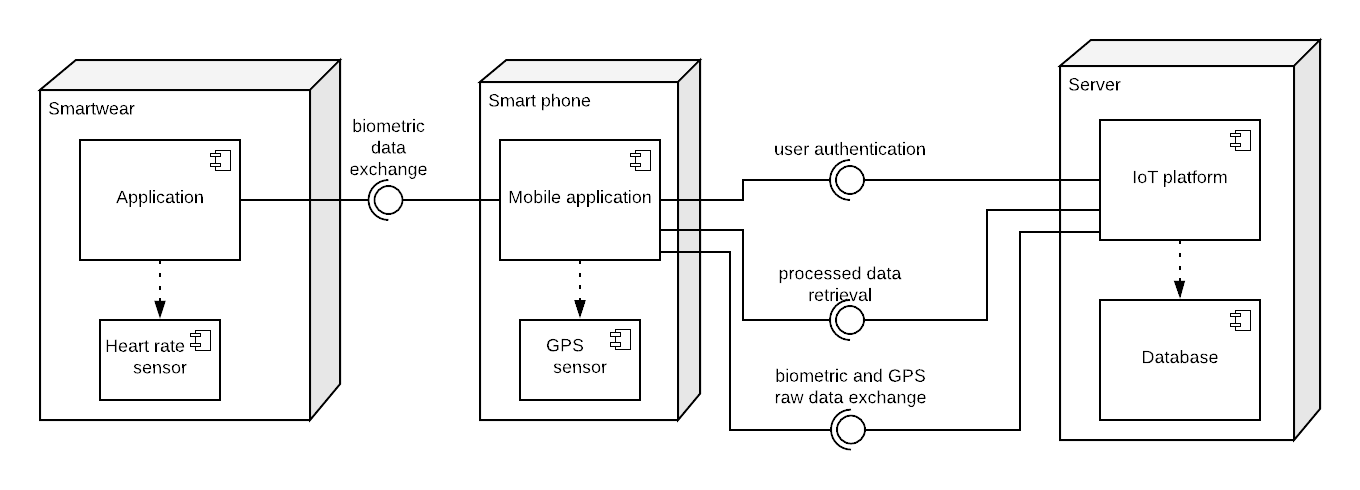
\includegraphics[width=\textwidth]{component.png}}
    \caption{Component diagram of the designed IoT solution}
\end{figure}

Depending on the number and complexity of the features in the future, it is also possible to introduce a web client in order to make the smartphone APP lighter and easier to navigate.

The watch communicates with the phone application over Bluetooth, with the watch application acting as a server, providing information for the client phone application.
The phone application connects to the server using the phone's Internet connection.

\section{PoC implementation}

I started by implementing a simple Android application that acts as a server for incoming Bluetooth connections from paired devices.
This was fairly straightforward since Android's documentation is up to date and there is a large community of developers for this OS.

The next step was to choose and integrate a smartwatch.

Initially 

I looked at multiple vendors' popularity based on market share and affordability, their documentation to see how good their development support is and whether or not they have public APIs for development.

According to Statista.com~\ref{fig:watch_market_share}, the most popular are Apple watches, followed by Samsung, Fitbit and other vendors.

\begin{figure}[h]
    \tmpframe{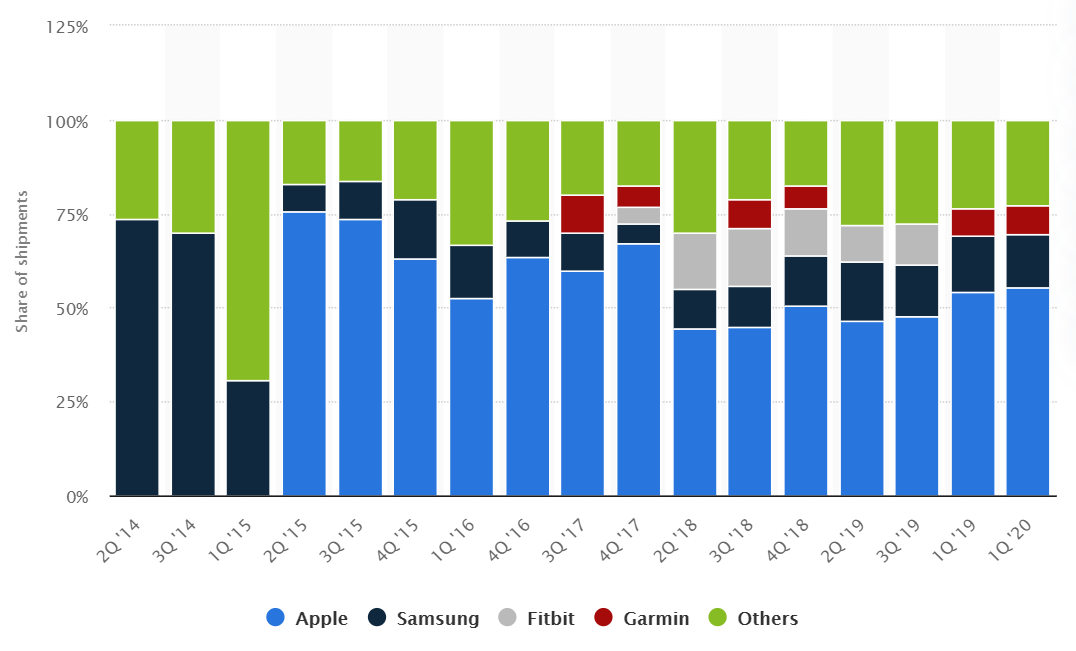
\includegraphics[width=\textwidth]{smartwatch_market_share.png}}
    \caption{Market share of smartwatch unit shipments worldwide from the 2Q'14 to 1Q '20*, by vendor~\cite{watch_market_share}.}
    \label{fig:watch_market_share}
\end{figure}

While Apple has a crushing lead on all other vendors, buying a unit just for development is not an option for me because of their high prices.
This is why I chose the Samsung Activity Watch.

Samsung watches run Tizen OS, which has public APIs, extensive documentation, tutorials and a large community.
This is why I was surprised to find out how difficult it is to develop for this watch.
The watch needs to be connected over the local network to the Tizen Studio IDE; the tutorial for this~\cite{tizen_connect_tutorial} omits the important step of enabling developer options when working with Bluetooth, so that the device does not disconnect when trying to use the Bluetooth API.
The tutorial also doesn't mention that Bluetooth should not only be disabled, but has to be turned off, on, and off again in order to connect.

Working with Bluetooth itself was tricky as well since their guide~\cite{tizen_bluetooth_guide} explicitly says that it should be implemented in the main thread, but then the app refuses to connect, and when I finally found a working sample application~\cite{tizen_bluetooth_sample}, its Bluetooth functionality was divided into different threads.

When implementing the watch's communication with the Android phone, another surprise was the missing step of asking for permissions to access the heart rate sensor~\cite{tizen_sensor_tutorial}.

When my application could finally both measure heart rate and send string data to the Android phone, I attempted to send the heart rate data, which the application successfully performed and then crashed, without an accessible crash log, stack trace, or any log that could shed light at the issue at hand.


